\documentclass{article}\usepackage[]{graphicx}\usepackage[]{xcolor}
% maxwidth is the original width if it is less than linewidth
% otherwise use linewidth (to make sure the graphics do not exceed the margin)
\makeatletter
\def\maxwidth{ %
  \ifdim\Gin@nat@width>\linewidth
    \linewidth
  \else
    \Gin@nat@width
  \fi
}
\makeatother

\definecolor{fgcolor}{rgb}{0.345, 0.345, 0.345}
\newcommand{\hlnum}[1]{\textcolor[rgb]{0.686,0.059,0.569}{#1}}%
\newcommand{\hlstr}[1]{\textcolor[rgb]{0.192,0.494,0.8}{#1}}%
\newcommand{\hlcom}[1]{\textcolor[rgb]{0.678,0.584,0.686}{\textit{#1}}}%
\newcommand{\hlopt}[1]{\textcolor[rgb]{0,0,0}{#1}}%
\newcommand{\hlstd}[1]{\textcolor[rgb]{0.345,0.345,0.345}{#1}}%
\newcommand{\hlkwa}[1]{\textcolor[rgb]{0.161,0.373,0.58}{\textbf{#1}}}%
\newcommand{\hlkwb}[1]{\textcolor[rgb]{0.69,0.353,0.396}{#1}}%
\newcommand{\hlkwc}[1]{\textcolor[rgb]{0.333,0.667,0.333}{#1}}%
\newcommand{\hlkwd}[1]{\textcolor[rgb]{0.737,0.353,0.396}{\textbf{#1}}}%
\let\hlipl\hlkwb

\usepackage{framed}
\makeatletter
\newenvironment{kframe}{%
 \def\at@end@of@kframe{}%
 \ifinner\ifhmode%
  \def\at@end@of@kframe{\end{minipage}}%
  \begin{minipage}{\columnwidth}%
 \fi\fi%
 \def\FrameCommand##1{\hskip\@totalleftmargin \hskip-\fboxsep
 \colorbox{shadecolor}{##1}\hskip-\fboxsep
     % There is no \\@totalrightmargin, so:
     \hskip-\linewidth \hskip-\@totalleftmargin \hskip\columnwidth}%
 \MakeFramed {\advance\hsize-\width
   \@totalleftmargin\z@ \linewidth\hsize
   \@setminipage}}%
 {\par\unskip\endMakeFramed%
 \at@end@of@kframe}
\makeatother

\definecolor{shadecolor}{rgb}{.97, .97, .97}
\definecolor{messagecolor}{rgb}{0, 0, 0}
\definecolor{warningcolor}{rgb}{1, 0, 1}
\definecolor{errorcolor}{rgb}{1, 0, 0}
\newenvironment{knitrout}{}{} % an empty environment to be redefined in TeX

\usepackage{alltt}
\usepackage[sc]{mathpazo}
\renewcommand{\sfdefault}{lmss}
\renewcommand{\ttdefault}{lmtt}
\usepackage[T1]{fontenc}
\usepackage{geometry}
\geometry{verbose,tmargin=2.5cm,bmargin=2.5cm,lmargin=2.5cm,rmargin=2.5cm}
\setcounter{secnumdepth}{2}
\setcounter{tocdepth}{2}
\usepackage[unicode=true,pdfusetitle,
 bookmarks=true,bookmarksnumbered=true,bookmarksopen=true,bookmarksopenlevel=2,
 breaklinks=false,pdfborder={0 0 1},backref=false,colorlinks=false]
 {hyperref}
\hypersetup{
 pdfstartview={XYZ null null 1}}

\makeatletter
%%%%%%%%%%%%%%%%%%%%%%%%%%%%%% User specified LaTeX commands.
\renewcommand{\textfraction}{0.05}
\renewcommand{\topfraction}{0.8}
\renewcommand{\bottomfraction}{0.8}
\renewcommand{\floatpagefraction}{0.75}

\makeatother
\IfFileExists{upquote.sty}{\usepackage{upquote}}{}
\begin{document}








The results below are generated from an R script.

\begin{knitrout}
\definecolor{shadecolor}{rgb}{0.969, 0.969, 0.969}\color{fgcolor}\begin{kframe}
\begin{alltt}
\hlcom{#^GSPC,}
\hlcom{#AAPL,MSFT,NVDA,TSM,ASML,AVGO,}
\hlcom{#GOOGL,META,DIS,TMUS,VZ,CMCSA,}
\hlcom{#AMZN,TSLA,HD,BABA,MCD,TM,}
\hlcom{#WMT,PG,KO,PEP,COST,FMX,}
\hlcom{#BHP,LIN,RIO,VALE,APD,SCCO}

\hlstd{a_all} \hlkwb{<-} \hlkwd{read.csv}\hlstd{(}\hlstr{"stockData.csv"}\hlstd{,} \hlkwc{sep}\hlstd{=}\hlstr{","}\hlstd{,} \hlkwc{header}\hlstd{=}\hlnum{TRUE}\hlstd{)}
\hlcom{#Convert adjusted close prices into returns:}
\hlstd{a} \hlkwb{<-} \hlstd{a_all[}\hlnum{1}\hlopt{:}\hlnum{60}\hlstd{,]} \hlcom{# Use 5 year data to train}
\hlstd{r} \hlkwb{<-} \hlstd{(a[}\hlopt{-}\hlnum{1}\hlstd{,}\hlnum{3}\hlopt{:}\hlkwd{ncol}\hlstd{(a)]}\hlopt{-}\hlstd{a[}\hlopt{-}\hlkwd{nrow}\hlstd{(a),}\hlnum{3}\hlopt{:}\hlkwd{ncol}\hlstd{(a)])}\hlopt{/}\hlstd{a[}\hlopt{-}\hlkwd{nrow}\hlstd{(a),}\hlnum{3}\hlopt{:}\hlkwd{ncol}\hlstd{(a)]}

\hlcom{#Compute mean vector:}
\hlstd{means} \hlkwb{<-} \hlkwd{colMeans}\hlstd{(r)}

\hlcom{#Compute variance covariance matrix}
\hlstd{covmat} \hlkwb{<-} \hlkwd{cov}\hlstd{(r)}

\hlcom{#Compute correlation matrix:}
\hlstd{cormat} \hlkwb{<-} \hlkwd{cor}\hlstd{(r)}

\hlcom{#Compute the vector of variances:}
\hlstd{variances} \hlkwb{<-} \hlkwd{diag}\hlstd{(covmat)}

\hlcom{#Compute the vector of standard deviations:}
\hlstd{stdev} \hlkwb{<-} \hlkwd{diag}\hlstd{(covmat)}\hlopt{^}\hlnum{.5}

\hlcom{#Plot the 31 assets on the space expected return against standard deviation}

\hlkwd{plot}\hlstd{(stdev, means,}
     \hlkwc{main}\hlstd{=}\hlstr{"Expected Return against Standard Deviation"}\hlstd{,}
     \hlkwc{xlab}\hlstd{=}\hlstr{"Standard Deviation"}\hlstd{,}
     \hlkwc{ylab}\hlstd{=}\hlstr{"Expected Return"}\hlstd{,}
     \hlkwc{xlim} \hlstd{=} \hlkwd{c}\hlstd{(}\hlnum{0}\hlstd{,} \hlnum{0.2}\hlstd{),}
     \hlkwc{ylim} \hlstd{=} \hlkwd{c}\hlstd{(}\hlnum{0}\hlstd{,} \hlnum{0.06}\hlstd{),}
     \hlkwc{pch}\hlstd{=}\hlnum{19}\hlstd{)}

\hlcom{#Assume equal allocation portfolio using the 30 stocks.}
\hlstd{new_means} \hlkwb{<-} \hlkwd{colMeans}\hlstd{(r[,}\hlopt{-}\hlnum{1}\hlstd{])}
\hlstd{new_covmat} \hlkwb{<-} \hlkwd{cov}\hlstd{(r[,}\hlopt{-}\hlnum{1}\hlstd{])}
\hlstd{new_cormat} \hlkwb{<-} \hlkwd{cor}\hlstd{(r[,}\hlopt{-}\hlnum{1}\hlstd{])}
\hlstd{new_variances} \hlkwb{<-} \hlkwd{diag}\hlstd{(new_covmat)}
\hlstd{new_stdev} \hlkwb{<-} \hlkwd{diag}\hlstd{(new_covmat)}\hlopt{^}\hlnum{.5}

\hlstd{number_of_stocks} \hlkwb{=} \hlnum{30}
\hlstd{ones_vector} \hlkwb{<-} \hlkwd{rep}\hlstd{(}\hlnum{1}\hlstd{, number_of_stocks)}
\hlstd{equal_weight_vector} \hlkwb{<-} \hlstd{ones_vector}\hlopt{/}\hlstd{number_of_stocks}

\hlstd{equal_varp} \hlkwb{<-} \hlkwd{t}\hlstd{(equal_weight_vector)} \hlopt \hlstd{new_covmat} \hlopt \hlstd{equal_weight_vector}
\hlstd{equal_sdp} \hlkwb{<-} \hlkwd{sqrt}\hlstd{(equal_varp)}

\hlstd{equal_Rp} \hlkwb{<-} \hlkwd{t}\hlstd{(equal_weight_vector)} \hlopt \hlstd{new_means}

\hlkwd{points}\hlstd{(equal_sdp, equal_Rp,} \hlkwc{pch} \hlstd{=} \hlnum{19}\hlstd{,} \hlkwc{lwd}\hlstd{=}\hlnum{5}\hlstd{,} \hlkwc{col}\hlstd{=}\hlstr{"red"}\hlstd{)}

\hlcom{#Assume minimum risk portfolio}

\hlstd{ones_vector} \hlkwb{<-} \hlkwd{rep}\hlstd{(}\hlnum{1}\hlstd{, number_of_stocks)}
\hlstd{inverse_new_covmat} \hlkwb{<-} \hlkwd{solve}\hlstd{(new_covmat)}
\hlstd{min_risk_weight_vector} \hlkwb{<-} \hlstd{inverse_new_covmat}  \hlopt \hlstd{ones_vector} \hlopt{/} \hlkwd{as.numeric}\hlstd{(}\hlkwd{t}\hlstd{(ones_vector)}  \hlopt \hlstd{inverse_new_covmat}  \hlopt \hlstd{ones_vector)}

\hlstd{min_risk_varp} \hlkwb{<-} \hlkwd{t}\hlstd{(min_risk_weight_vector)} \hlopt \hlstd{new_covmat} \hlopt \hlstd{min_risk_weight_vector}
\hlstd{min_risk_sdp} \hlkwb{<-} \hlkwd{sqrt}\hlstd{(min_risk_varp)}
\hlstd{min_risk_Rp} \hlkwb{<-} \hlkwd{t}\hlstd{(min_risk_weight_vector)} \hlopt \hlstd{new_means}

\hlkwd{points}\hlstd{(min_risk_sdp, min_risk_Rp,} \hlkwc{pch}\hlstd{=}\hlnum{19}\hlstd{,} \hlkwc{lwd}\hlstd{=}\hlnum{5}\hlstd{,} \hlkwc{col}\hlstd{=}\hlstr{"green"}\hlstd{)}

\hlkwd{legend}\hlstd{(}\hlstr{"topright"}\hlstd{,} \hlkwc{legend}\hlstd{=}\hlkwd{c}\hlstd{(}\hlstr{"Minimum Risk Portfolio"}\hlstd{,} \hlstr{"Equal Allocation"}\hlstd{,} \hlstr{"Individual stocks"}\hlstd{),}
       \hlkwc{col}\hlstd{=}\hlkwd{c}\hlstd{(}\hlstr{"green"}\hlstd{,} \hlstr{"red"}\hlstd{,}\hlstr{"black"}\hlstd{),}\hlkwc{pch} \hlstd{=} \hlnum{19}\hlstd{,}\hlkwc{fill} \hlstd{=}\hlkwd{c}\hlstd{(}\hlstr{"green"}\hlstd{,} \hlstr{"red"}\hlstd{,}\hlstr{"black"}\hlstd{),}\hlkwc{cex}\hlstd{=}\hlnum{0.8}\hlstd{)}
\end{alltt}
\end{kframe}

{\centering 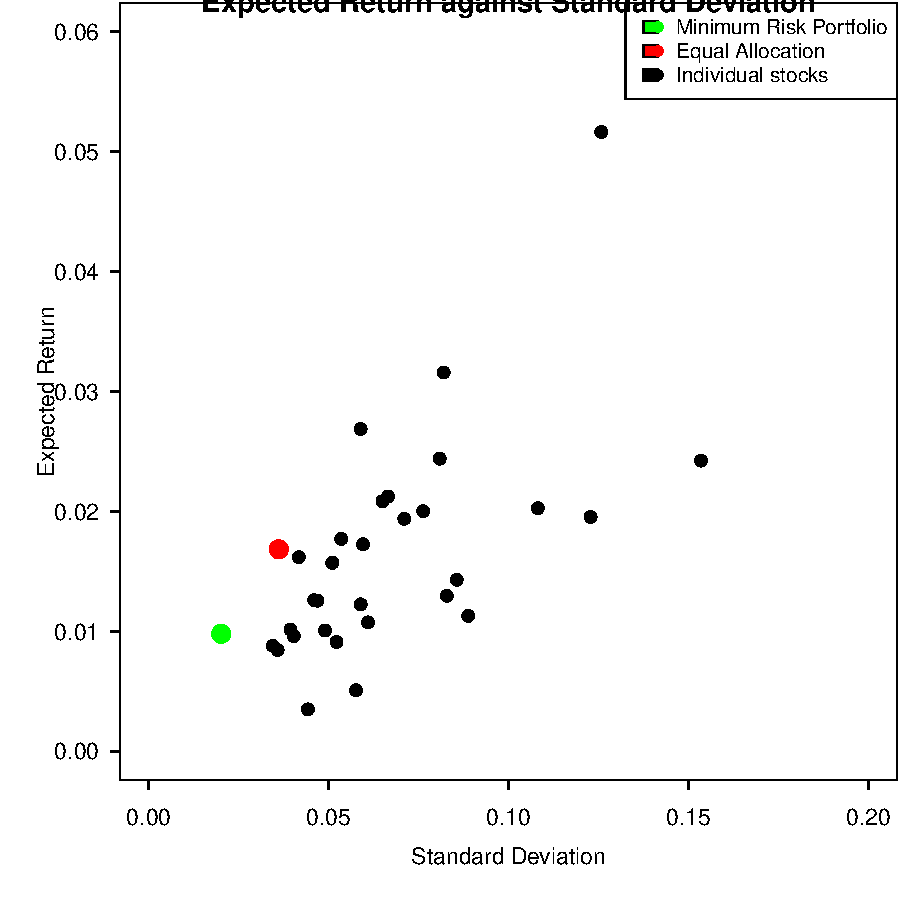
\includegraphics[width=.6\linewidth]{figure/part1-Rnwauto-report-1} 

}


\end{knitrout}

The R session information (including the OS info, R version and all
packages used):

\begin{knitrout}
\definecolor{shadecolor}{rgb}{0.969, 0.969, 0.969}\color{fgcolor}\begin{kframe}
\begin{alltt}
\hlkwd{sessionInfo}\hlstd{()}
\end{alltt}
\begin{verbatim}
## R version 4.2.2 (2022-10-31 ucrt)
## Platform: x86_64-w64-mingw32/x64 (64-bit)
## Running under: Windows 10 x64 (build 22621)
## 
## Matrix products: default
## 
## locale:
## [1] LC_COLLATE=English_United States.utf8  LC_CTYPE=English_United States.utf8   
## [3] LC_MONETARY=English_United States.utf8 LC_NUMERIC=C                          
## [5] LC_TIME=English_United States.utf8    
## 
## attached base packages:
## [1] stats     graphics  grDevices utils     datasets  methods   base     
## 
## other attached packages:
## [1] quantmod_0.4.21 TTR_0.24.3      xts_0.13.0      zoo_1.8-11      pdfetch_0.2.8  
## [6] shiny_1.7.4    
## 
## loaded via a namespace (and not attached):
##  [1] Rcpp_1.0.10       highr_0.10        jquerylib_0.1.4   bslib_0.4.2      
##  [5] pillar_1.9.0      compiler_4.2.2    later_1.3.0       tools_4.2.2      
##  [9] digest_0.6.31     evaluate_0.20     memoise_2.0.1     jsonlite_1.8.4   
## [13] lubridate_1.9.2   lifecycle_1.0.3   tibble_3.2.1      timechange_0.2.0 
## [17] lattice_0.20-45   pkgconfig_2.0.3   rlang_1.1.0       cli_3.6.0        
## [21] yaml_2.3.7        curl_5.0.0        xfun_0.37         fastmap_1.1.1    
## [25] knitr_1.42        dplyr_1.1.1       httr_1.4.5        sass_0.4.5       
## [29] generics_0.1.3    vctrs_0.6.1       grid_4.2.2        tidyselect_1.2.0 
## [33] fontawesome_0.5.0 glue_1.6.2        R6_2.5.1          fansi_1.0.4      
## [37] XML_3.99-0.14     rmarkdown_2.20    tidyr_1.3.0       purrr_1.0.1      
## [41] magrittr_2.0.3    promises_1.2.0.1  ellipsis_0.3.2    htmltools_0.5.4  
## [45] mime_0.12         xtable_1.8-4      httpuv_1.6.9      utf8_1.2.3       
## [49] cachem_1.0.7
\end{verbatim}
\begin{alltt}
\hlkwd{Sys.time}\hlstd{()}
\end{alltt}
\begin{verbatim}
## [1] "2023-04-08 13:53:09 PDT"
\end{verbatim}
\end{kframe}
\end{knitrout}


\end{document}
